\documentclass[a4paper, 12pt]{article}
\usepackage{temp}
\usepackage{epsfig,graphicx,subfigure,amsthm,amsmath, float, xcolor, changepage, mathtools, textcomp, hyperref, bm, amssymb, tcolorbox, tikz, setspace}
\usepackage{array}
\usepackage[shortlabels]{enumitem}
\usepackage[stable]{footmisc}
\usepackage{xepersian}
\settextfont[Scale=1]{XBZar}
%\setdigitfont{XBZar}
\setlatintextfont[Scale=0.9]{Times New Roman}
\hypersetup{
	colorlinks=true,
	urlcolor=blue!70!black
}

\doublespacing
\begin{document}
\handout
{هوش مصنوعی}
{نیم‌سال اول ۰۱\lr{-}۰۰}
{دکتر محمدحسین رهبان}
{دانشکده مهندسی کامپیوتر}
{تمرین ششم - بخش دوم}
{محمدجواد هزاره}
{98101074}
\noindent
\\[-6em]
\section*{سوال ۱}
مقدار خروجی $f$ با توجه به عکس زیر برابر
$\frac{e}{1+e}$
خواهد بود.
\begin{figure}[H]
	\centering
	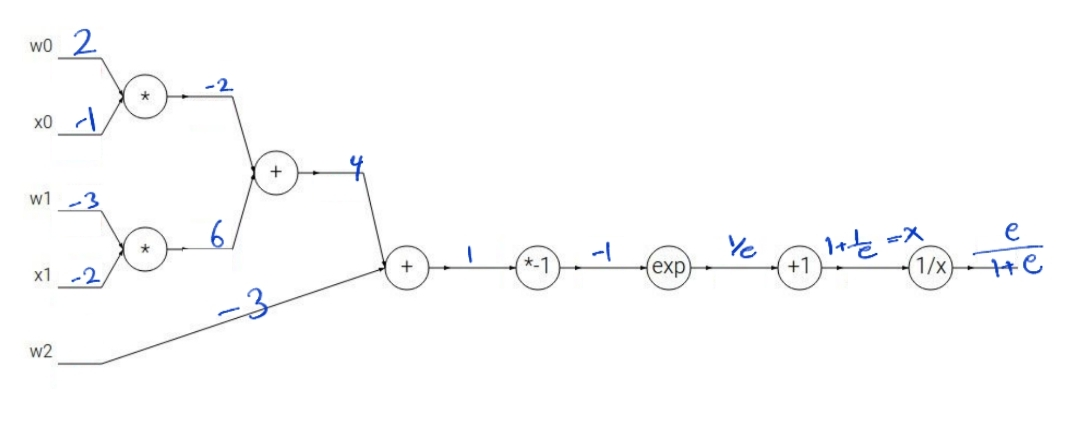
\includegraphics[width=0.9\textwidth]{forward.jpg}
\end{figure}
\noindent
برای محاسبه‌ی مشتق خروجی نسبت به $w$ها نیز مطابق تصویر با استفاده از
\lr{backpropagation}
خواهیم داشت: (که $X$ ورودی آخرین راس است.)
\begin{figure}[H]
	\centering
	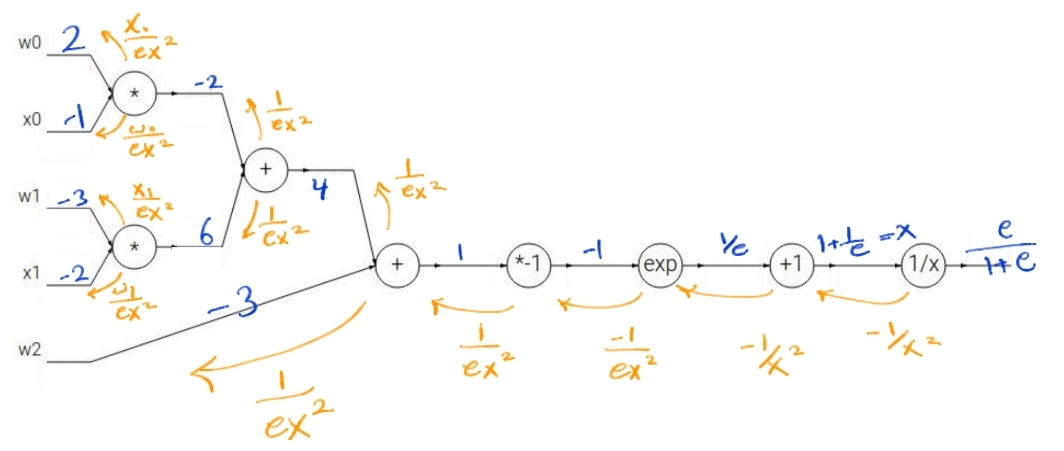
\includegraphics[width=0.9\textwidth]{backpropagation.jpg}
\end{figure}
\[
\begin{dcases}
	\frac{\partial f}{\partial w_0} = \frac{x_0}{eX^2} = \frac{-e}{(1+e)^2} \\[0.4em]
	\frac{\partial f}{\partial w_1} = \frac{x_1}{eX^2} = \frac{-2e}{(1+e)^2} \\[0.4em]
	\frac{\partial f}{\partial w_2} = \frac{1}{eX^2} = \frac{e}{(1+e)^2}
\end{dcases}
\]
\end{document}



